\section{实验2:AI标签对个性化广告效果的影响}
实验1的结果表明,即使在未明确告知广告来源的情况下,参与者仍能够在一定程度上区分AI生成和人类创作的广告。这表明AI生成广告在语言特征或表达方式上具有独特之处,使其与人类创作的广告有所不同。然而,消费者不仅会根据广告文本的语言特征来推测广告的来源,还可能受到明示信息的影响。当广告明确标注为“AI生成”时,这一信息是否会进一步影响消费者对广告的感知和接受度?换言之,AI 作为广告的生成者,是否会影响个性化广告的说服力?这一问题尚未得到充分探讨。

个性化广告的有效性依赖于心理契合度(psychological fit),即消费者是否认为广告内容与自身需求高度相关。在这一过程中,感知相似性(perceived similarity) 是个性化广告影响消费者态度的核心心理机制 \citep{teeny2021review}。然而,现有研究较少直接测量感知相似性在个性化广告说服过程中的作用,因此本研究首先验证该变量是否确实在个性化广告与消费者态度之间起中介作用。另一方面,人工智能(AI)因缺乏社交属性,往往被认为是心理距离(psychological distance) 更远的主体\citep{kim2020artificial}。心理距离的增加可能导致消费者AI生成广告的感知相似性降低,从而影响个性化广告的说服效果 \citep{ahn2021ai}。换言之,即便AI生成的广告内容符合消费者特征,其个性化效果仍可能因信息来源的影响而受到削弱。基于此,实验2采用两步研究设计,首先验证感知相似性在个性化广告中的关键作用(实验 2a)。实验 2b 在实验 2a 的基础上,进一步引入 AI 标签,以探讨广告来源(AI 生成 vs. 人类创作)是否会影响个性化广告的效果。

\subsection{实验2a:感知相似性的中介探究}
\subsubsection{方法}
(1)被试

实验通过见数平台发布,共 162 名参与者 自愿参加本研究。其中,19 名参与者因未通过注意力检测被剔除,最终保留 143 名有效被试(年龄范围 = 18-48 岁,\textit{M} = 23.83 岁,\textit{SD} = 4.25),其中女性 96 名。每名受试者在完成实验后获得 2 元人民币 作为报酬。

(2)实验材料

本实验采用研究一实验2中的实验材料(\ref{study1-substudy2-methods}),涉及两类产品(薯片与电脑),分别针对尽责性与开放性两个人格特质进行个性化广告设计。对于每种产品-人格特质的组合,实验材料均包含:中性广告(来自社交媒体的原始广告,不包含特定个性化元素);个性化广告(基于该中性广告生成的针对性广告内容,以匹配目标人格特质)。每位参与者需依次观看四组广告(即两种产品 × 两种人格特质),其中每组包含一则中性广告和一则个性化广告。广告呈现顺序随机。观看后,参与者需对每组广告进行评价。

(3)问卷测量

大五人格量表和广告说服效果,测量方法与研究一实验2一致(\ref{study1-substudy2-methods})。除此以外,本实验引入感知相似性 \ref{li2016does},参与者需对以下条目进行评分:“广告的内容符合我的兴趣和需求”,“广告看起来是否像是特地为我设计的”,“广告是否呈现了与我的个性特征相匹配的信息。” 所有测量均采用likert-7点量表(1=完全不同意,7=完全同意),以评估参与者对个性化广告的感知相似程度。

\subsubsection{结果}

在研究一实验2的个性化广告有效的基础上,本实验主要关注感知相似性的中介作用。具体而言,采用 SPSS PROCESS Macro(Model 4) 进行中介效应分析。其中,自变量分别为开放性得分和尽责性得分,因变量为对应个性化广告的说服效果(即开放性个性化广告的效果和尽责性个性化广告的效果),中介变量为感知相似性。

首先,针对开放性维度设计的个性化广告场景(如图\ref{fig:openness-mediation_model}),结果表明开放性得分显著正向预测感知相似性(\textit{b} = 0.8091, \textit{SE} = 0.0892, \textit{t} = 9.0705, \textit{p} < .001),说明高开放性个体更倾向于认为开放性个性化广告符合自身需求。其次,感知相似性显著正向预测广告的说服效果(\textit{b} = 0.5070, \textit{SE} = 0.0335, \textit{t} = 15.1340, \textit{p} < .001)。此外,在控制感知相似性后,开放性得分对广告说服效果的直接效应仍显著(\textit{b} = 0.1289, \textit{SE} = 0.0573, \textit{t} = 2.2482, \textit{p} = .0253)。中介效应分析表明,感知相似性的间接效应为 0.4102,其 95\% 置信区间为 [0.3143, 0.5141],不包含 0,表明感知相似性在开放性个性化广告的个性化效果中起到了中介作用。

\begin{figure}[H] % htbp 让 LaTeX 决定合适的位置
    \centering
    \begin{tikzpicture}[
        node distance=3.5cm,
        every node/.style={align=center, minimum height=1cm, font=\small}, 
        every path/.style={draw, -{Latex[round]}, thick}
    ]
        % 定义变量节点
        \node[draw, rounded corners] (X) {开放性 \\ (自变量)};
        \node[draw, rounded corners, above=of X, xshift=5cm] (M) {感知相似性 \\ (中介变量)};
        \node[draw, rounded corners, right=of X, xshift=5cm] (Y) {个性化说服效果 \\ (因变量)};
        
        % 画箭头,并直接在线上标注路径系数
        \path (X) -- node[midway, above, sloped] {\( 0.8091^{***} \)} (M);
        \path (M) -- node[midway, above, sloped] {\( 0.5070^{***} \)} (Y);
        \path (X) -- node[midway, below, sloped] {\( 0.1289^{*}, 95\% CI=[0.0160, 0.2418] \)} (Y);
        
        % 间接效应标注
        \node[above=0.2cm of M, align=center, font=\small] {
            \textbf{间接效应}: 0.4142, 95\% CI=[0.3143, 0.5141]
        };
        
    \end{tikzpicture}
    \caption{开放性-中介效应模型示意图}
    \label{fig:openness-mediation_model} % 交叉引用时使用 \ref{fig:mediation_model}
\end{figure}

类似地,在针对尽责性维度设计的个性化广告场景中(如图\ref{fig:conscientiousness-mediation_model}),尽责性得分同样显著正向预测感知相似性(\textit{b} = 0.4918, \textit{SE} = 0.0720, \textit{t} = 6.8338, \textit{p} < .001),说明高尽责性个体更倾向于认为尽责性个性化广告符合自身需求。同样,感知相似性显著正向预测广告的说服效果(\textit{b} = 0.4984, \textit{SE} = 0.0298, \textit{t} = 16.7066, \textit{p} < .001)。在控制感知相似性后,尽责性得分对广告说服效果的直接效应仍显著(\textit{b} = 0.1015, \textit{SE} = 0.0392, \textit{t} = 2.5906, \textit{p} = .0101)。中介效应分析表明,感知相似性的间接效应为 0.2451,其 95\% 置信区间为 [0.1566, 0.3388],不包含 0,说明感知相似性在尽责性个性化广告的个性化效果中同样起到了部分中介作用。

\begin{figure}[H] % htbp 让 LaTeX 决定合适的位置
    \centering
    \begin{tikzpicture}[
        node distance=3.5cm,
        every node/.style={align=center, minimum height=1cm, font=\small}, 
        every path/.style={draw, -{Latex[round]}, thick}
    ]
        % 定义变量节点
        \node[draw, rounded corners] (X) {尽责性 \\ (自变量)};
        \node[draw, rounded corners, above=of X, xshift=5cm] (M) {感知相似性 \\ (中介变量)};
        \node[draw, rounded corners, right=of X, xshift=5cm] (Y) {个性化说服效果 \\ (因变量)};
        
        % 画箭头,并直接在线上标注路径系数
        \path (X) -- node[midway, above, sloped] {\( 0.4918^{***} \)} (M);
        \path (M) -- node[midway, above, sloped] {\( 0.4984^{***} \)} (Y);
        \path (X) -- node[midway, below, sloped] {\( 0.1015^{*}, 95\% CI=[0.0244, 0.1785] \)} (Y);
        
        % 间接效应标注
        \node[above=0.2cm of M, align=center, font=\small] {
            \textbf{间接效应}: 0.2351, 95\% CI=[0.1566, 0.3388]
        };
        
    \end{tikzpicture}
    \caption{尽责性-中介效应模型示意图}
    \label{fig:conscientiousness-mediation_model} % 交叉引用时使用 \ref{fig:mediation_model}
\end{figure}


上述分析表明,感知相似性在个性化广告的说服效果中起到了显著的中介作用。即,高开放性/高尽责性的个体在观看与其人格特质匹配的个性化广告时,更倾向于认为广告和自己的相似性,从而增强广告的说服力。此结果验证了感知相似性是个性化广告有效性的关键心理机制,为后续探讨 AI 作为广告生成者是否会影响该机制提供了理论基础。

\subsection{实验2b:AI标签影响的实证研究}
\subsubsection{方法}

本实验采用 $2 \times 2$ 的混合实验设计,其中广告创作者(GPT-4 vs. 人类专家)作为被试间变量,个性化程度(个性化 vs. 非个性化)作为被试内变量。实验旨在探讨 AI 作为广告创作者是否会影响个性化广告的说服效果,并考察个性化广告与信息来源之间的交互作用。


(1)被试

实验通过见数平台发布,共304名参与者自愿参加研究。经注意力检测筛选后,共剔除16名不合格的参与者,最终纳入288名有效被试(年龄范围 = 20-69岁,$\textit{M} = 31.45$,$\textit{SD} = 9.27$),其中146名为女性。所有被试在完成实验后均获得2元人民币作为报酬。

(2)实验材料

本实验选取小米手机(广告中匿名为「M手机」) 在社交媒体上的真实广告文本,并基于该广告文本指导GPT-4生成个性化版本。生成后确保所有广告文本具有相同的产品信息。采用的提示词(prompt)是:“请根据下面的社交媒体上的中性广告内容,修改为两个版本的个性化广告文案,使得目标消费者购买意愿增强,尽管其他消费者不一定喜欢:
1. 针对高外倾性消费者的版本。
2. 针对低外倾性消费者的版本。”

(3)实验流程

在阅读广告材料之前,所有参与者都会根据自己所分配到的条件,被告知特定的广告创造者(cover story)。如果参与者被分配到GPT-4,对广告创作者的描述为:“M手机是一款即将推向市场的智能手机。在本研究中,我们希望了解您对两段广告文案的反馈,以便根据用户反馈优化广告设计。您即将看到的广告文案是由 GPT-4 生成的。GPT-4 是 OpenAI 开发的一款先进的人工智能模型,专门用于理解和生成文本。” 如果参与者被分配到人类专家组,对广告创作者的描述则为:“M 手机是一款即将推向市场的智能手机。在本研究中,我们希望了解您对两段广告文案的反馈,以便根据用户反馈优化广告设计。您即将看到的广告文案是由经验丰富的市场营销专家撰写的,他们擅长创意广告设计和理解消费者心理。” 接下来,所有被试需阅读两则广告文案(一则为针对高外倾设计的广告,一则为低外倾设计的广告),广告呈现顺序随机。参与者需在阅读完每则广告后,完成问卷效果的测量,两则广告评价完后完成人格量表和性别、年龄等人口统计学信息。

(4)问卷测量

a. 说服效果。采用研究一实验2的测量方法(\ref{study1-substudy2-methods})。被试需对广告的说服力进行评分,共包含 5 个题目,采用 1-5 点李克特量表 评分,最终计算平均值作为说服效果得分。

b. 外倾性人格量表:本实验关注外倾性这一人格特质,因此从 \citet{john1991big} 编制的 大五人格量表(BFI-44) 中筛选与外倾性相关的 8 道题目,要求被试根据自身情况进行评分(1=完全不符合,5=完全符合)。

\subsubsection{结果}
首先,为计算个性化水平,本研究以被试的外倾性得分中位数为划分标准,将外倾性得分大于或等于中位数的被试归类为高外倾群体,低于中位数的被试归类为低外倾群体。在广告呈现方面,对于高外倾个体而言,观看专门针对高外倾性设计的广告被定义为个性化广告,而观看针对低外倾性设计的广告则被定义为非个性化广告。相应地,对于低外倾个体而言,观看针对低外倾性设计的广告被定义为个性化广告,而观看针对高外倾性设计的广告则被定义为非个性化广告。

为了探讨广告创作者标签(GPT-4 vs. 人类专家)对个性化广告说服效果的影响,本研究采用了 $2 \times 2$ 的重复测量方差分析,其中个性化(个性化 vs. 非个性化)作为被试内变量,广告创作者标签(GPT-4 vs. 人类专家)作为被试间变量。结果表明(如图\ref{fig:Source_personalization}),个性化与广告创作者标签之间的交互作用达到显著水平,$\textit{F}(1,112) = 6.866, \textit{p} = .010, \eta_p^2 = .058$,表明个性化广告的效果受到广告创作者标签的影响,即标注不同来源的广告在个性化说服力上的表现存在显著差异。进一步的简单效应分析显示,在被标注为人类专家创作的广告中,个性化广告的说服力显著高于非个性化广告(均值差异 = -0.171, 标准误 = 0.092, $\textit{p} = .028$,95\% CI = [0.010, 0.035]),说明当广告被标注为由人类专家撰写时,个性化广告的优势得以体现,受众更容易接受个性化内容。然而,在被标注为 GPT-4 生成的广告中,个性化广告与非个性化广告的说服力差异并不显著(均值差异 = 0.166, 标准误 = 0.090, $\textit{p} = .102$,95\% CI = [-0.023, 0.344]),说明当广告明确标注为 AI 生成时,个性化广告的优势效应被削弱。这一结果表明,即使广告文本内容完全相同,仅仅是信息来源的标注差异,就足以影响个性化广告的说服效果,进一步验证了AI作为信息源在个性化广告中的重要影响。

\begin{figure}[H]
    \centering
    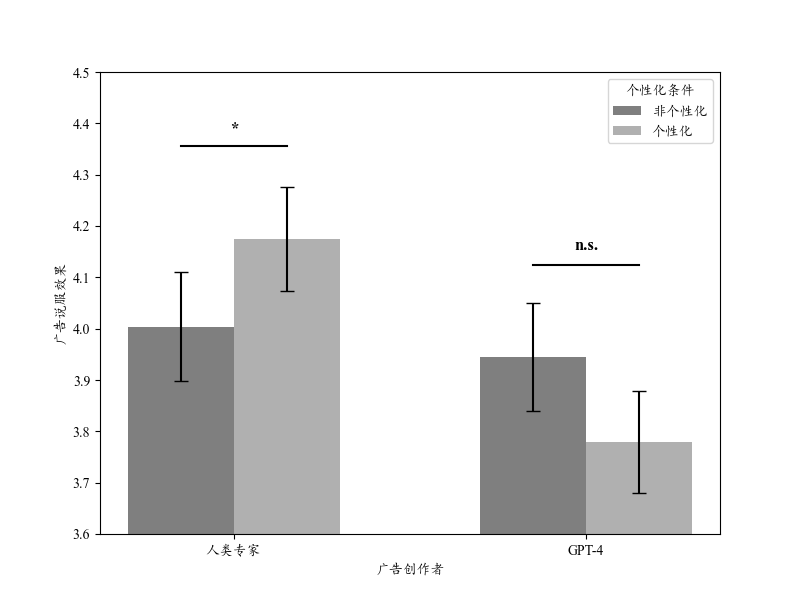
\includegraphics[width=1\linewidth]{Image/Study4-Source_Personalization.png}
    \caption{\label{fig:Source_personalization}广告创作者对个性化广告说服力的影响}
\end{figure}